\begin{figure}[H]
    \begin{center}
        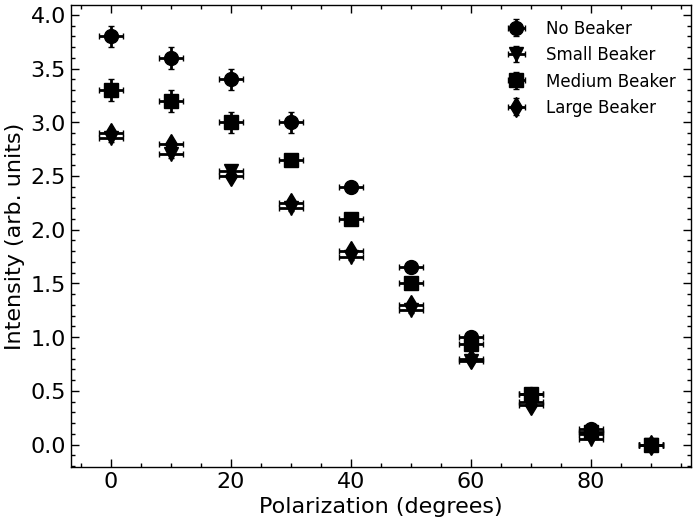
\includegraphics[width=\columnwidth]{../figures/no_water.png}
    \end{center}
    \caption{Intensity vs. Polarization for varying beaker sizes with no water.}
    \label{fig:no_water}
\end{figure}

\begin{figure}[H]
    \begin{center}
        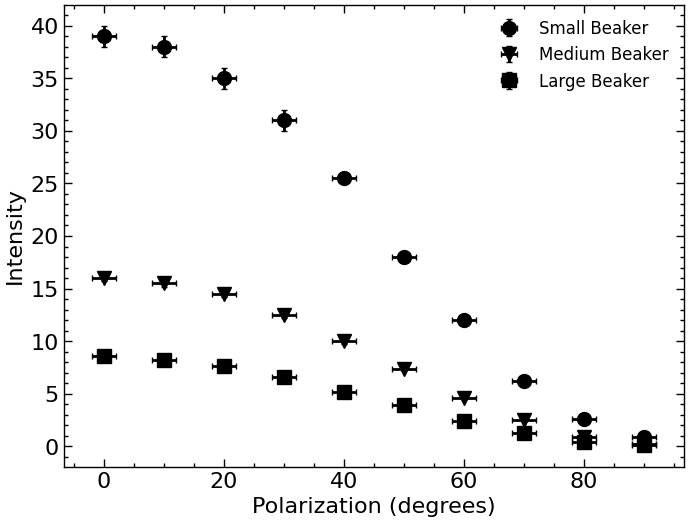
\includegraphics[width=\columnwidth]{../figures/water.png}
    \end{center}
    \caption{Intensity vs. Polarization for varying beaker sizes with water.}
    \label{fig:water}
\end{figure}

\begin{figure}[H]
    \begin{center}
        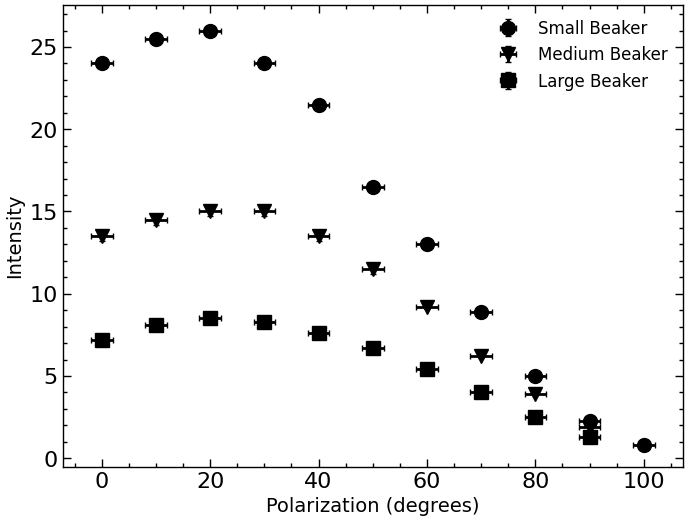
\includegraphics[width=\columnwidth]{../figures/solution1.png}
    \end{center}
    \caption{Intensity vs. Polarization for varying beaker sizes with solution 1.}
    \label{fig:solution1}
\end{figure}

\begin{figure}[H]
    \begin{center}
        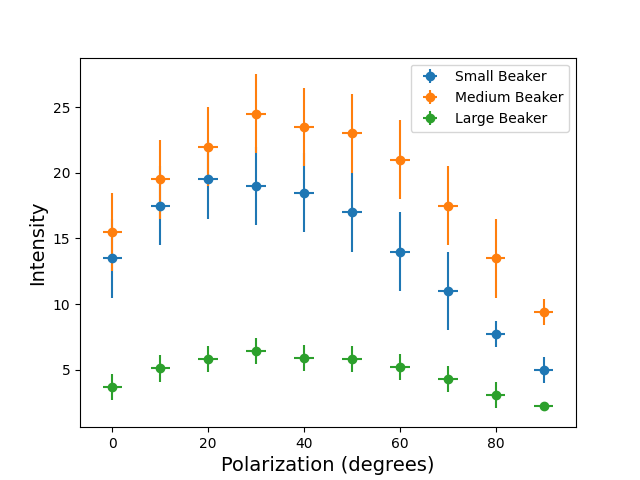
\includegraphics[width=\columnwidth]{../figures/solution2.png}
    \end{center}
    \caption{Intensity vs. Polarization for varying beaker sizes with solution 2.}
    \label{fig:solution2}
\end{figure}

\begin{figure}[H]
    \begin{center}
        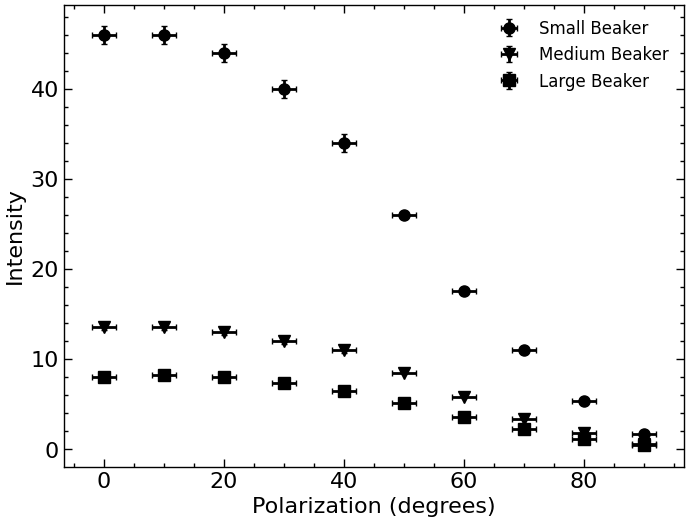
\includegraphics[width=\columnwidth]{../figures/solution3.png}
    \end{center}
    \caption{Intensity vs. Polarization for varying beaker sizes with solution 3.}
    \label{fig:solution3}
\end{figure}

\begin{figure}[H]
    \begin{center}
        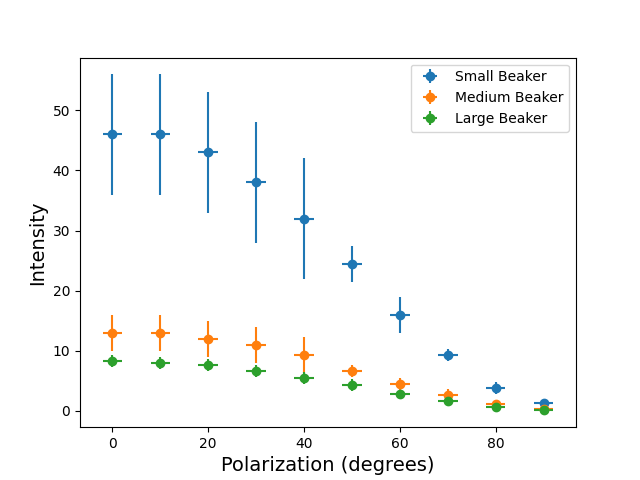
\includegraphics[width=\columnwidth]{../figures/solution4.png}
    \end{center}
    \caption{Intensity vs. Polarization for varying beaker sizes with solution 4.}
    \label{fig:solution4}
\end{figure}

\newpage
Each of the following graphs show the phase shift as a function of sugar concentration in water, with each separate graph containing data from one beaker size. 
The phase shifts were found by fitting the intensity vs. polarization data to a cosine function. By representing phase shift versus sugar concentration,
we can quantify how the polarization of light changes as a function of sugar concentration in water.

\begin{figure}[H]
    \begin{center}
        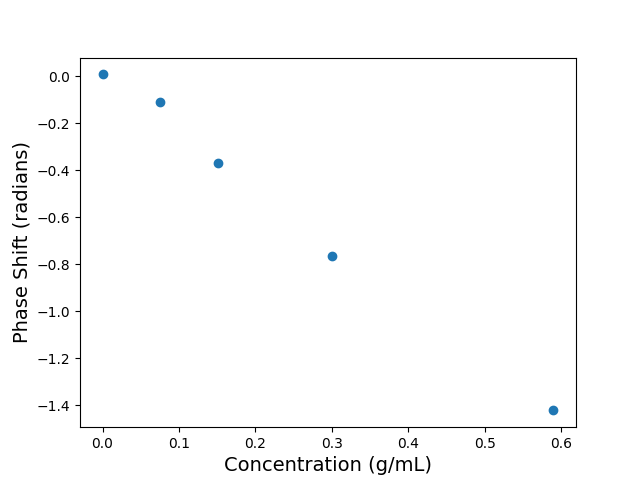
\includegraphics[width=\columnwidth]{../figures/large_beaker_phase_shifts.png}
    \end{center}
    \caption{This graph shows the phase shifts for large beaker.}
    \label{fig:large_beaker_phase_shifts}
\end{figure}

\begin{figure}[H]
    \begin{center}
        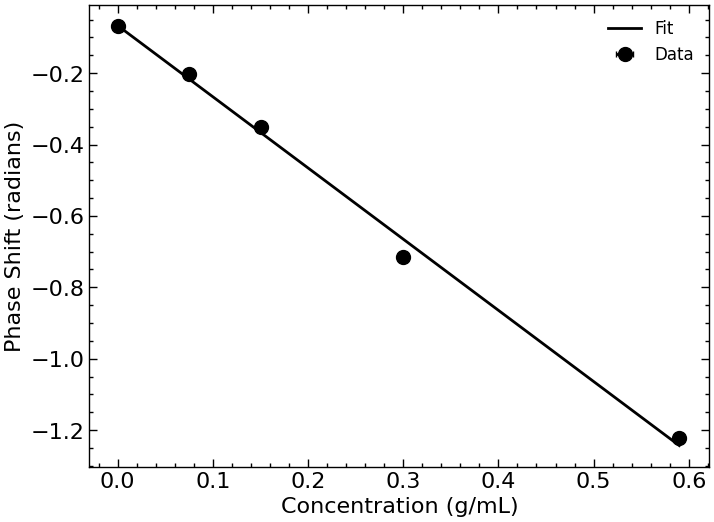
\includegraphics[width=\columnwidth]{../figures/medium_beaker_phase_shifts.png}
    \end{center}
    \caption{Phase shifts for medium beaker.}
    \label{fig:medium_beaker_phase_shifts}
\end{figure}

\begin{figure}[H]
    \begin{center}
        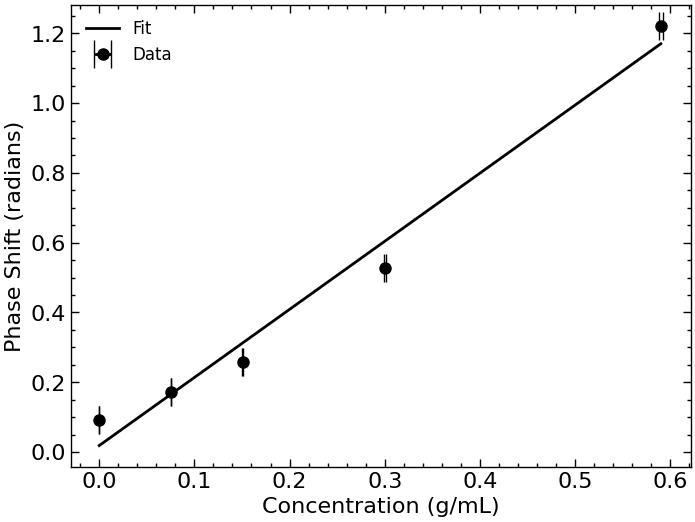
\includegraphics[width=\columnwidth]{../figures/small_beaker_phase_shifts.png}
    \end{center}
    \caption{Phase shifts for small beaker.}
    \label{fig:small_beaker_phase_shifts}
\end{figure}